As not all of the dataset samples were of the same quality it was important to first filter the dataset to remove the bad imaging samples. Even with the normal conditions many of the images contain a lot of background, that creates a big background vs. foreground class imbalance (see Figure \ref{fig:bad-smaples}a). Overexposure is also a typical problem, that gives samples of a too high intensity and without details inside the nucleus (see Figure \ref{fig:bad-smaples}b, c). Lastly, underexposure is as problematics as an overexposure (see Figure \ref{fig:bad-smaples}d).

\begin{figure}[H]
	\begin{center}
		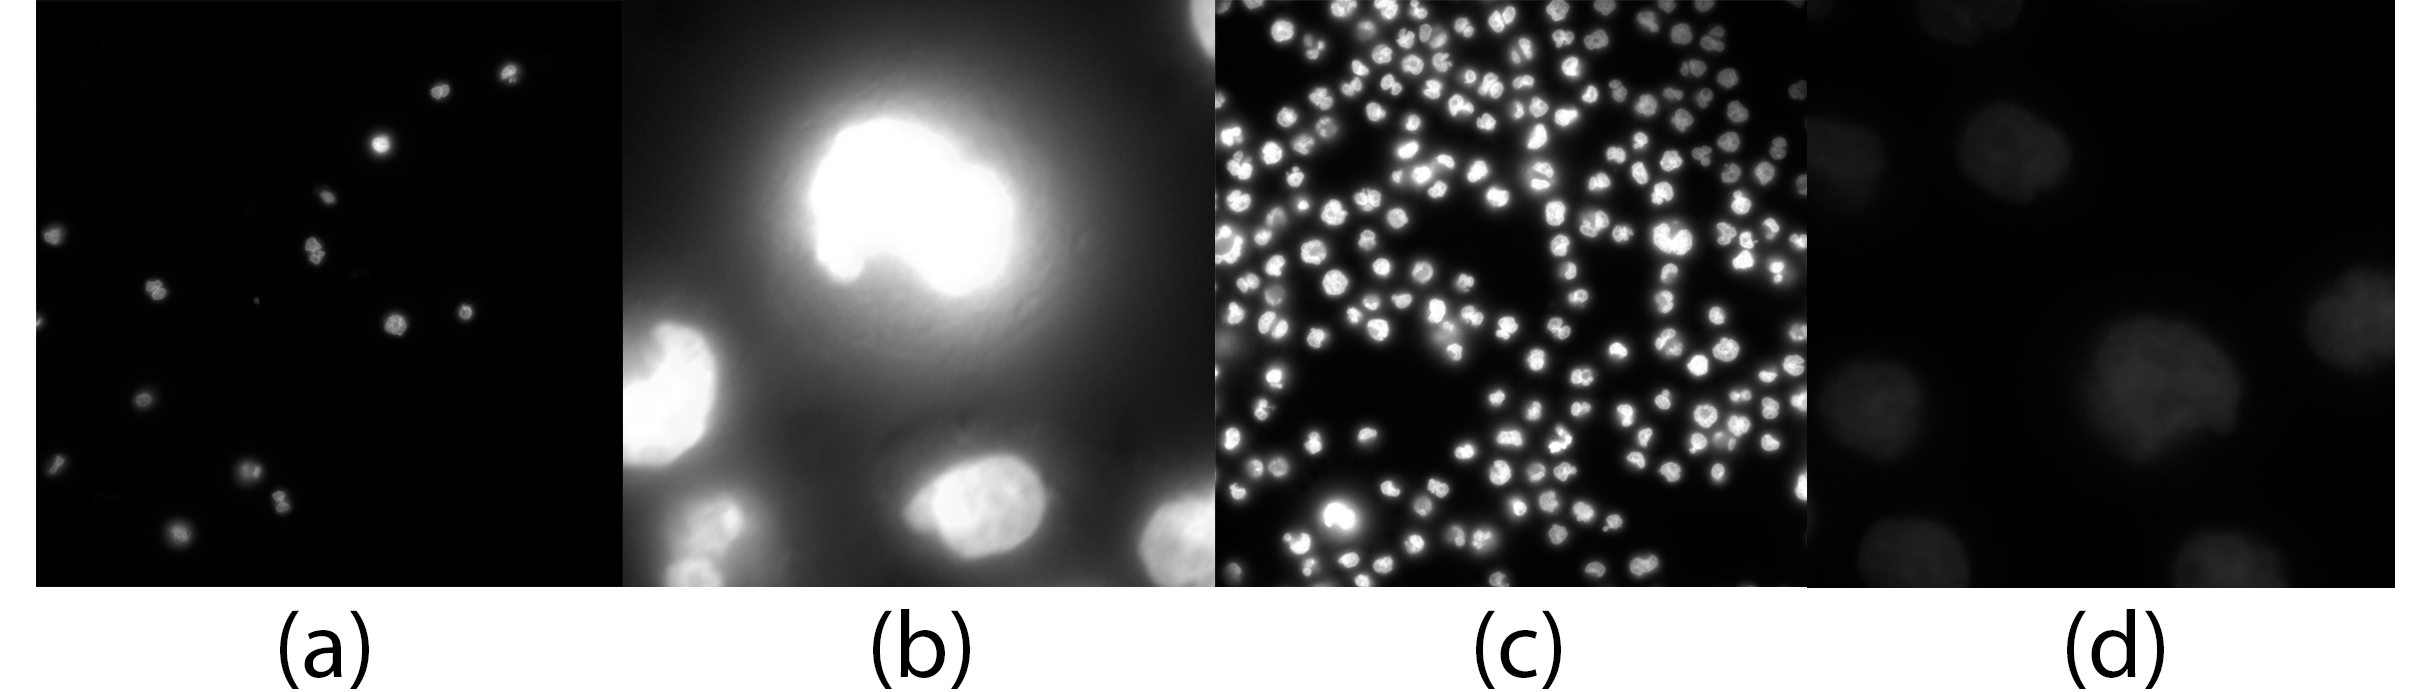
\includegraphics[width=0.6\linewidth]{bilder/nuclei/filter-out.png}
		\caption{Samples to be filtered out}\label{fig:bad-smaples}
	\end{center}
\end{figure}

Once the images have been filtered out, they were normalized to have the values between 0 and 1.